\chapter{Scala}
Wir haben uns entschieden, das Programm in Scala zu schreiben, einer Sprache, die bereits schon im Jahr 2001 von Martin Odersky entwickelt wurde, jedoch erst seit kurzem einen großen Bekanntheitsgrad erlangt hat. Grund dafür ist der Hype um die sogenannte \textit{funktionale Programmierung} und das Bedürfnis, Anwendungen nebenläufig zu entwickeln.
Wir möchten nun zu Beginn die Gründe nennen, warum Scala sich als moderne Programmiersprache anbietet, die sogar von Javas Hauptentwickler James Gosling als bevorzugte Java-Alternative betitelt wurde \footnote{James Gosling wurde auf einer Konferenz gefragt, welche Programmiersprache er heutzutage anstelle von Java auf der JVM nutzen würde, worauf er entschieden mit ``Scala'' antwortete --- \url{http://www.adam-bien.com/roller/abien/entry/java_net_javaone_which_programming}}.

\section{Laufzeit-Umgebung}
Scala ist wie Java eine Programmiersprache, die zu Bytecode kompiliert wird. Dieser Bytecode wird dann von der \textit{Java Virtual Machine} (\texttt{JVM}) benutzt um daraus Maschinencode zu erstellen. Die JVM ist mittlerweile auf sehr vielen Rechnern installiert und sogar das Android Betriebssystem setzt auf eine Variante der JVM (\texttt{Dalvik}).

Die JVM hat den großen Vorteil, dass sie mittlerweile seit 20 Jahren aktiv entwickelt wird und die gesamte Java-Umgebung besonders im Enterprise Bereich eingesetzt wird. Das Resultat ist ein sehr stabiles und vor allem perfomantes System, das aus dem heutigen IT-Markt nicht mehr wegzudenken ist.

\section{Bibliotheken}
Scala wird also nicht zu irgendeinem Bytecode kompiliert, sondern zu Java-Bytecode, um genau zu sein. Dies hat den großen Vorteil, dass man neben der JVM-Unterstützung auch auf etablierte Java Bibliotheken zugreifen kann. Beispielsweise ist der Einsatz von Google GSON\footnote{Link zu der Projektseite von Google GSON: \url{https://github.com/google/gson}}, das das Serialisieren von Objekten in JSON und zurück ermöglicht, über Scala so möglich, wie auch über Java.

So ist es dann auch kaum überraschend, dass der Einsatz von den üblichen Java Bibliotheken in Scala möglich ist. Ein Beispiel ist \texttt{JavaFX}, welches seit Java 8 Teil des \textit{Java Development Kit} (\texttt{JDK}) ist.

\section{JavaFX und ScalaFX}
Um die Oberfläche (User Interface) zu gestalten, nutzt man heute Bibliotheken, die meistens so komplex sind, dass ihnen ganze Werke gewidmet werden. Wir haben uns für JavaFX entschieden, welches durch den Wrapper ScalaFX angesprochen wird. Was diese Bibliotheken machen und auszeichnet, wird in den folgenden Abschnitten erklärt.

\subsection{JavaFX}
JavaFX 8 ist der offzielle Nachfolger von Swing. Zu Beginn sollte es eine Scriptssprache werden, jedoch wurde dieser Fokus mit Version 2 aufgegeben und JavaFX wurde zu der GUI Bibliothek, wie man sie heute nutzt. In der aktuellen Version 8 (welcher der direkte Nachfolger von Version 2 ist und wegen der Einbindung in das JDK 8 diesen Versionssprung vollzogen hat), wurde die Bibliothek um wichtige Komponenten erweitert und bietet die folgendenden Vorteile:

\begin{description}
\item[Scene Graph]\hfill\\
JavaFX ist besonders leicht zu entwickeln, da es auf den \texttt{Scene Graph} setzt. Der Scene Graph ist eine Baumstruktur, bei der die Elemente hierachisch angeordnet werden. Elemente im Scene Graph sind vom Type \texttt{Node} ~\cite{ProJavaFX8}. Wenn man also beispielsweise einen Button auf der Bildfläche platzieren möchte, dann hat man ein Button Objekt, welches von \texttt{Node} erbt

\begin{figure}[!htb]
    \centering
      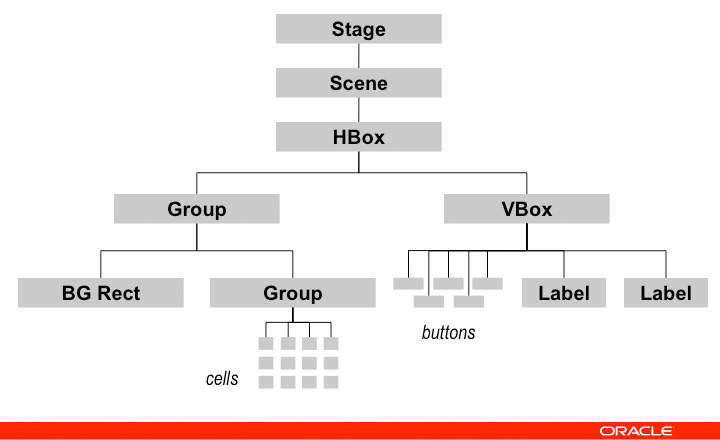
\includegraphics[width=0.75\linewidth]{scene-graph}
    \caption{Darstellung der Baumstruktur im Scene Graph}
    \label{fig:scene-graph}
\end{figure}

Ein Vorteil ist, dass man so Objekte gruppieren kann und dadurch Operationen auf der Gruppe ausführen kann. So wird bei einer Verschiebe-Operation (auch \textit{Translation} genannt) jedes Element in der Gruppe verschoben, was den Code lesbarer und wartbarer macht.\\
Außerdem ist somit eine zum Eltern Element relative Positionierung möglich.

\item[Klares MVC]\hfill\\
Bei JavaFX wird das Konzept für das Design in einer separaten Datei, einer \textbf{FXML} Datei geführt. So muss man das Layout nicht im Code generieren. Im Abschnitt zu FXML~\ref{sec:fxml} wird dies ausführlicher beschrieben.

\item[Styling über CSS]\hfill\\
Neben der Trennung von Ablauf, Logik und Gestaltung nach dem \textit{MVC}-Prinzip, lässt sich das Styling durch eine CSS-ähnliche Syntax durchführen, was das Gestalten von Oberflächen durch Designer ermöglicht. Es wird jedoch eine leicht abgewandelte Syntax verwendet. Das Setzen der Textfarbe auf rot (\texttt{\#ff0000} im RGB-Farbraum) wird durch die CSS-Syntax
\begin{verbatim}
.button: {
  -fx-color: #f00;
}
\end{verbatim}
ermöglicht. Man erkennt, dass das Präfix \texttt{-fx-} vor dem CSS-Befehl steht.

\item[Properties und Bindings]\hfill\\
Das Koppeln von von Eigenschaften einer Klasse an eine andere Klasse ist ein tolles Feature, welches das Entwickeln von komplexen Anwendungen noch weiter vereinfacht. Intern wird das \texttt{Observable}-Interface benutzt, die Komponenten zu aneinander zu binden.

Um Bindings und die dazu benutzten Properties besser zu verstehen, verweisen wir auf die sehr gute Zusammenfassung auf \cite{JavaBeginner-Binding}
\end{description}

\subsection{ScalaFX}
ScalaFX ist eine \textit{Domain Specifig Language}\footnote{Bei einer \texttt{DSL} handelt es sich um eine formale Sprache, die ein bestimmtes Problemfeld abdeckt. In dem Fall von ScalaFX handelt es sich um eine \textit{UI DSL}, die als Wrapper um JavaFX gelegt wird.} (\texttt{DSL}) für JavaFX. Als \texttt{DSL} bietet ScalaFX syntaktischen Zucker für die JavaFX--Bibliothek, und die folgenden Vorteile:

\begin{description}
\item[Lesbare Bind-Ausdrücke]\hfill\\
Binding und Properties gehören zu den tollen Funktionen, die JavaFX bietet, jedoch ist die Syntax teilweise sehr umständlich.
\paragraph{Beispiel:} Wenn man 3 Rechtecke hat (\texttt{rect1}, \texttt{rect2} und \texttt{reckt3}) und man möchte, dass das Rechteck \texttt{rect1} so hoch ist, wie \texttt{rect2} und \texttt{rect3}, dann bindet man die Höhe von \texttt{rect1} an die summierte Höhe von \texttt{rect2} und \texttt{rect3}.

\underline{Scala}:
\begin{lstlisting}[language=scala,caption=Scala Beispiel Code für natürliche Bindings,numbers=none]
rect1.height <== rect2.height + rect3.height
\end{lstlisting}

\underline{Java}:
\begin{lstlisting}[language=Java,caption=Das selbe Beispiel in Java,numbers=none]
rect1.heightProperty().bind(rect2.heightProperty().add(rect3.heightProperty()))
\end{lstlisting}

Der Scala Code ist wesentlich intuitiver und lesbarer, was genau der Sinn dieser \texttt{DSL} ist. Das Beispiel stammt aus \cite{ProJavaFX8} (Seite 574f.).

\item[Angepasste Animations Syntax]\hfill\\
Da Animationen ein wichtiger Bestandteil von JavaFX sind, wurde die Syntax wesentlich verbessert. Auch hier möchten wir uns an \cite{ProJavaFX8} halten und Scala Code mit Java Code vergleichen.

\underline{Scala}:
\begin{lstlisting}[language=scala,caption=Scala Beispiel für eine einface Animation,numbers=none]
Timeline(at (3 s) {radius -> 0}).play()
\end{lstlisting}

\underline{Java}:
\begin{lstlisting}[language=Java,caption=Das selbe Beispiel in Java,numbers=none]
KeyValue collapse = new KeyValue(circle.radiusProperty(),0);
new Timeline(new KeyFrame(Duration.seconds(3), collapse))
  .play();
\end{lstlisting}

\item[Typsichere APIs]\hfill\\
Ein Vorteil von Scala, wie wir noch kennen lernen werden, ist dass die Sprache \textit{statisch typisiert} ist. ScalaFX ist garantiert \textit{typsicher}, was zur Folge hat, dass Fehler bereits beim Kompilieren auftreten und nicht erst zur Laufzeit zu Fehlern führen wird. ~\cite{TypesAndProgrammingLanguages}

\item[Interoperabilität zwischen ScalaFX und JavaFX]\hfill\\
ScalaFX liegt wie ein Wrapper um JavaFX und bietet Funktionen an, die die Arbeit mit JavaFX erleichtern. Dies wird dadurch vereinfacht, dass man ganz einfach zwischen JavaFX und ScalaFX wechseln kann. Ein besonders hilfreiches Konzept sind hierbei \textit{Implizite Konvertierungen}. So kann man beispielsweise eine \texttt{javafx.scene.Shape.button} an eine Methode übergeben, die ein \texttt{scalafx.scene.Shape.button} als Argument erwartet.
\end{description}

Da es sich bei ScalaFX primär um syntaktische Verbesserungen handelt, kann man argumentieren, dass die Benutzung obsolet ist. Wir haben uns bewusst für die Integration entschieden, da wir näher an der Scala Syntax bleiben wollten und die Lesbarkeit von Source-Code für uns ein wichtiger Aspekt ist\footnote{Eine Interessante Diskussion zu diesem Thema findet man auch hier \url{http://stackoverflow.com/a/22744881}}.


\subsection{FXML}\label{sec:fxml}
Wenn man sich mit den Entwicklung von Swing auskennt, dann weiß man, dass man alle darstellbaren Objekte im Code selber generiert und gestaltet. Möchte man diese dann später ändern, so muss man sich mit dem Programmcode auseinander setzen und hier die Syntax nachvollziehen und Änderungen über die Programmiersprache vornehmen.

Dieser Ansatz ist in JavaFX auch möglich, jedoch hat dies den Nachteil, dass die Oberfläche durch den teilweise umständlichen Programmierstil beschrieben wird. Außerdem müssen sich Oberflächen-Gestalter in die Programmiersprache einarbeiten.\\
FXML ist eine auf \texttt{XML} basierende Sprache, dass die Struktur des Layouts beschreibt. Man kann das FXML Layout ganz einfach auslagern, also in einer separaten Datei speichern, sodass Anwendungs-Logik und die Präsentationsschicht getrennt sind, so wie im \texttt{Model-View-Control} Pattern gefordert.

Dadurch, dass das Layout über den Scene\textbf{graph} organisiert wird, bietet sich XML durch seine verschachtelten Tags an, diese Knotenstruktur abzubilden. Somit wird diese Struktur auch gleichzeitig \textbf{transparent}.\\
FXML wird nicht kompiliert, somit können Änderungen ohne vorheriges Rekompilieren direkt getestet werden.\\
Ein großer Vorteil ist, dass man einzelnen Knoten \texttt{ID}s und \texttt{Class}es zuteilen kann, wie in HTML. Diese lassen sich dann über CSS stylen. Hierbei wird eine leicht veränderte CSS-Syntax verwendet, aber jeder der sich in der Webgestaltung auskennt, wird sich hier schnell zurecht finden. Neben dem Stylen von Elementen ist die \textbf{Lokalisierung} des Inhalts heutzutage auch extrem wichtig, da der Softwaremarkt mittlerweile kaum mehr auf einen Sprachraum beschränkt ist. Hier bietet FXML eingebaute Features, die diese Lokalisierung sehr einfach ermöglichen.\\
Und da JavaFX das Laden und verarbeiten von FXML Dateien erlaubt, kann man auch mit anderen JVM--Sprachen, wie in unserem Fall Scala, FXML nutzen. Wir haben jedoch eine zusätzliche Library genutzt, die das Benutzen und Arbeiten mit FXML Dateien erleichtert: ScalaFXML~\cite{ScalaFXML}.

Zuletzt muss man in Verbindung mit FXML noch den Scene Builder\footnote{Der Scene Builder ist mittlerweile Open Source und kann hier herunter geladen werden \url{http://gluonhq.com/labs/scene-builder/}. Weitere Informationen findet man noch auf der mittlerweile archivierten Oracle Seite unter \url{http://www.oracle.com/technetwork/java/javase/downloads/javafxscenebuilder-info-2157684.html}} nennen. Dieses Tool erleichtert die Gestaltung von einfachen User Interfaces, indem Elemente per Drag \& Drop platziert werden können und man somit eine Oberfläche gestalten kann, ohne sich genauer mit dem FXML Code auseinander setzen zu müssen. Das Programm hat uns am Anfang geholfen, die Syntax besser zu verstehen und die Elemente besser zu platzieren. Da wir in unserer Arbeit jedoch immer öfter Kleinigkeiten im Layout anpassen mussten, haben wir im Verlauf immer mehr auf den Scene Builder verzichtet, da die Anpassung einer ID, oder Größe oder das Einfügen eine Buttons händisch tatsächlich schnell geht und der Scene Builder nicht fehlerfrei funktionierte. Bei unser wurde die Menüzeile des Scene-Builders (von wo aus man das Layout beispielsweise als native Anwendung ohne Logik testen kann) durch das Menü unserer Anwendung überschrieben \footnote{Der Fehler wird hier beschrieben: \url{https://bugs.openjdk.java.net/browse/JDK-8089659}. Wir haben das Tag \texttt{useSystemMenuBar} genutzt, um auf OSX die native Menüzeile zu nutzen, was das Layout natürlicher macht.}.

\section{Grundlegendes und Syntax}
Die Programmiersprache Scala ist sehr komplex und die Sprache hier vorzustellen und zu erklären würde den Umfang dieser Ausarbeitung sprengen. Dennoch möchten wir einige Grundlegende Spracheigenschaften vorstellen, sodass man den später vorgestellten Code besser nachvollziehen kann.\\
Man kann zwar Scala Code schreiben, der sehr an Java Code erinnert, jedoch wird davon abgeraten. Einer der grundlegenden Ansätze\footnote{Siehe: \url{http://www.scala-lang.org/documentation/getting-started.html}} ist, dass man sich die elementaren Konzepte von Scala verinnerlicht und Code schreibt, der funktioniert. Man kann dann immer noch die komplexeren Eigenschaften der Sprache lernen.

Da dies das erste Programm ist, das wir in Scala geschrieben haben, kann man bestimmt viele Sachen besser machen, wenn man entsprechend Erfahrung hat. Dennoch haben wir probiert, viele der tollen Features zu nutzen, die Scala bietet.

Viele der folgenden Beispiel kann man in der \textbf{REPL} (\texttt{Read-Evaluate-Print-Loop}) testen. Die REPL ist so etwas wie eine interaktive Console, in der man Scala Code testen und ausprobieren kann. Da wir diese für unsere Projektarbeit nicht direkt benötigten, aber eine tolle Möglichkeit darstellt um Scala Code zu testen, verweisen wir auf die tolle Beschreibung von \cite{GettingStartedWithTheScalaREPL}

\subsection{Typinferenz}
Scala ist eine statisch typisierte Sprache. Das bedeutet, dass eine Variable von einem Typ ist, der sich auch nicht ändert. In Java gibt man den Typ bei der Deklaration direkt mit an. Wenn man Beispielsweise einen Variable \texttt{helloWorld} vom Type \texttt{String} hat, die den Wert \texttt{Hello World} hat, dann wird dies wie folgt angegeben:

\begin{lstlisting}[language=Java,numbers=none]
String helloWorld = "Hello World";
\end{lstlisting}

In Scala kann man den Typ weglassen, den die Variable hat, dieser wird vom Compiler beim Kompilieren ausgewertet. Es reicht also, wenn man

\begin{lstlisting}[language=Scala,numbers=none]
val helloWorld = "Hello World"
\end{lstlisting}

schreibt.\\
Wenn man möchte, so kann man den Typ dennoch mit angeben, das sieht dann wie folgt aus:

\begin{lstlisting}[language=Scala,numbers=none]
val helloWorld: String = "Hello World"
\end{lstlisting}

In den obigen Beispielen fällt auf, dass es ein Schlüsselwort gibt, das es in Java so nicht gibt: \texttt{val}. Außerdem muss man kein Semikolon an das Ende der Zeilen machen. Wie so oft in Scala gilt für das Semikolon: Muss man nicht, kann man aber.\\
Was es mit dem Schlüsselwort \texttt{val} auf sich hat, möchten wir im nächsten Abschnitt aufzeigen.

\subsection{Values und Variablen}
Das \texttt{val} steht für einen Value, also einen unveränderlichen Wert. Scala ist eine funktionale Programmiersprache. Einer der wichtigen Ansätze hierbei ist die \textit{Immuntability}, also die \textit{Unveränderlichkeit} von Werten. Man möchte bei nebenläufigen Operationen keine Werte haben, die von anderen Threads verändert werden können. Um dies zu vermeiden, benutzt man unveränderliche Werte, also \textbf{Values}. Dies entspricht einer \texttt{final}-Variable in Java.\\
Das Code-Fragment

\begin{lstlisting}[language=Scala,numbers=none]
val number = 1
number = 2
\end{lstlisting}

führt also zu dem Fehler:
\begin{verbatim}
error: reassignment to val
\end{verbatim}

An dieser Stelle benötigt man also eine Variable \texttt{var}:

\begin{lstlisting}[language=Scala,numbers=none]
var number = 1
number = 2
\end{lstlisting}

\subsection{Methoden}
Methoden werden ähnlich wie in Java geschrieben. Sie haben einen Rückgabetype und eine ParameterListe. Wir wollen uns im folgenden eine sehr einfache Methode angucken:

\begin{lstlisting}[language=Scala]
def isLarge(value: Int): Boolean = {
  if (value > 15)
    true
  else
    false
}
\end{lstlisting}

Die Methode mit dem Namen \texttt{isLarge} nimmt also als Parameter einen \texttt{Integer}, den man mit dem Namen \texttt{value} anspricht. Die Methode hat Rückgabetyp \texttt{Boolean}.

Die Methode zeigt auch schon einige Besonderheiten an Scala. Man erkennt, dass das Schlüsselwort \texttt{return} nicht angegeben werden muss. In Java würde man \texttt{return true} und \texttt{return false} schreiben müssen \footnote{Man kann if Statements wie einen ternären Operator nutzen, siehe: \cite{ScalaCookbook} Section 3.6 --- \textit{Using the if Construct Like a Ternary Operator}} \footnote{Return Statements sollten vermieden werden, wie in \cite{ScalaInDepth} Section 2.2.1 --- \textit{Don't use return} beschrieben}. Dies hat den Hintergrund, dass \textbf{jeder Ausdruck ausgewertet wird} und somit etwas zurück gegeben wird. Wenn man nichts zurückgeben möchte, so gibt man \texttt{Unit} an. Unit gibt an, dass man mit dem Ergebnis, das zurückgegeben wird, nichts anfangen kann und kommt dem \texttt{void} in Java nahe. Beispielsweise die \texttt{println()} Methode hat den Rückgabetyp \texttt{Unit}.

Um das obige Beispiel noch klarer zu machen, speichern wir den von dem If-Statement zurückgegebenen Wert in einem Value, den wir dann zurück geben werden:

\begin{lstlisting}[language=Scala]
def isLarge2(value: Int): Boolean = {
  val isValueLarger = (if (value > 15) true else false)

  isValueLarger
}
\end{lstlisting}

Die beiden Methoden machen beide das Selbe. Wenn wir die Methode in der \texttt{REPL} testen, bekommen wir folgendes Ergebnis:

\begin{verbatim}
  scala> def isLarge(value: Int): Boolean = {
       |   val isValueLarger = (if (value > 15) true else false)
       |
       |   isValueLarger
       | }
  isLarge: (value: Int)Boolean

  scala> isLarge(9)
  res0: Boolean = false

  scala> isLarge(20)
  res1: Boolean = true
\end{verbatim}

Wir werden die Methode \texttt{isLarge} im Weiteren Verlauf noch weiter benutzen um die Funktionen von Scala hervorzuheben.

\subsection{Strings}

Das Arbeiten mit Strings in Scala ist sehr einfach und es gibt einige sehr nützliche Funktionen, die dafür sorgen, dass der Code nicht nur lesbarer, sondern auch leichter zu warten ist.

Das Konkatenieren von Strings und Variablen in Java ist sehr praktisch und einfach, man fügt diese einfach durch ein \texttt{+} Zeichen aneinander.

\begin{lstlisting}[language=Java,numbers=none]
System.out.println("Is the number " + number + " a large number: " isLarge(number));
\end{lstlisting}

In Scala muss man sich keine Gedanken mehr um das Konkatenieren an sich machen, der gleiche Code wie oben sieht so aus:

\begin{lstlisting}[language=Scala,numbers=none]
println(s"Is the number $number a large number: ${isLarge(number)}")
\end{lstlisting}

Das Weglassen von \texttt{System.out} ist kein Fehler, sondern ein Scala nicht nötig. Durch das Voransetzen von \texttt{s} an den String, kann man Variablen durch \texttt{\$} ganz einfach einsetzen. Ausdrücke werden durch \texttt{\$\{\}} eingefügt, müssen also geklammert werden.

\subsubsection{Mehrzeilige Strings mit Sonderzeichen}
Ein weiteres tolles Feature ist, dass man mehrzeilige Strings nicht manuell umbrechen muss. Durch das Setzen von 3 Anführungszeichen zu Beginn des Strings, kann man den String einfach umbrechen:

\begin{lstlisting}[language=Scala]
val multiLineString = """This
     |is
     |an
     |example""".stripMargin
println(multiLineString)
\end{lstlisting}

Dies ergibt die Ausgabe:

\begin{verbatim}
This
is
an
example
\end{verbatim}

Eine tolle Beschreibung für diese Funktionalität gibt es in \cite{ScalaCookbook} unter Section 1.2.

Eine weitere syntaktische Neuerung ist, dass die Methode \texttt{stripMargin()} ohne die Klammern aufgerufen wird. Dies ist in Scala möglich, wenn eine Methode keine Argumente erwartet.

Tatsächlich ist es möglich, dass man sogar den Punkt zwischen dem String (also dem Objekt) und der Methode weglässt. Dies bezeichnet man als \textit{Postfix Operator Notation}, ein Feature, was Code teilweise sehr lesbar und schön macht, aber auch zu unerwartetem Verhalten führen kann \footnote{Diese Stackoverflow Diskussion klärt einige dieser Fragen, setzt jedoch voraus, dass man sich mit der Scala Syntax auskennt: \url{http://stackoverflow.com/questions/13011204/scalas-postfix-ops}}

\subsection{Getter \& Setter}\label{sec:getter-and-setter}
Die Nutzung von Getter-- und Setter--Methoden Zugriff auf die Attribute eines Objekts ist gang und gäbe in Java. In Scala wird auf die Felder wie zugegriffen, als wären diese public, obwohl dies nicht der Fall ist. Scala generiert beim Kompilieren die Methoden, die den Zugriff auf die Variablen erlauben. Ein Beispiel\footnote{Das Beispiel stammt von \url{http://dustinmartin.net/getters-and-setters-in-scala/}} soll dies veranschaulichen:

\begin{lstlisting}[language=Scala, caption=Beispiel Klasse Person]
class Person() {
  var name = ""
  var age = 0
}
\end{lstlisting}

Da die Klasse keine Methoden hat könnte man meinen, dass der Zugriff auf \texttt{name} und \texttt{age} nicht möglich ist. Jedoch wurden die Getter-- und Setter--Methoden von Scala automatisch erstellt und man kann nun auf die Felder zugreifen:

\begin{lstlisting}[language=Scala]
person = new Person()

println(person.age)
println(person.name)
\end{lstlisting}

Man kann die Getter und Setter auch überschreiben, siehe hierzu \cite{ScalaCookbook} Section 4.6 und die Quelle dieses Beispiels.

\subsection{For--Schleifen}\label{sec:for-loops}

Schleifen sind ein elementares Konstrukt aus der Programmierung. Bei den For--Schleifen wird dabei meistens eine Zählvariable benutzt, die bis zu einem gewissen Wert zählt und mit der man dann Sachen machen kann. Ein klassisches Beispiel ist das Befüllen eines Arrays mit Werten.

\begin{lstlisting}[language=Java,caption=Typische For--Schleife aus der Java Programmierung]
for (int i = 0; i <= array.length; i++) {
  array[i] = i * i;
}
\end{lstlisting}

Bei dem obigen Beispiel wird das Quadrat der Zählvariablen gespeichert. Da man hierbei manuell prüfen muss, wie lang das Array-Objekt ist \texttt{array.length}. Um typische Fehler zu vermeiden (beispielsweise \texttt{ArrayIndexOutOfBoundsException}), wurden Iteratoren eingeführt und man durchläuft Listen etc. durch For-Each Schleifen. Wenn man jedoch einen Index-Zugriff ermöglichen will, so benötigt man wieder eine Zählvariable.

\begin{lstlisting}[language=Java]
int i = 0;
for (int element : array) {
  System.out.println(i + ": " + element); // Gibt Index und enthaltenes Element aus
  i++;
}
\end{lstlisting}

Da die Zählvariable \texttt{i} somit \textit{varriabel} sein müsste, gibt es in Scala einen anderen Ansatz. Man kann durch ein Schleifenkonstrukt wie folgt, die obige Ausgabe erreichen:

\begin{lstlisting}[language=Scala]
val array = new Array(1,2,3,4,5,6)
for (i <- 0 until array.length) {
  println(s"$i: ${array(i)"})
}
\end{lstlisting}

Wie man erkennt, greift man nicht mehr über \texttt{array[i]} auf ein Element in dem Array zu, sondern über \texttt{array(i)}. Ansonsten zählt man die i Variable hoch. Man kann auch eine For-Each Schleife kreiren, so wird aus dem Beispiel oben:

\begin{lstlisting}[language=Scala,caption=For--Each in Scala]
var i = 0
for (element <- array) {
  println(s"$i: $element)
  i += 1
}
\end{lstlisting}

Die Syntax sollte nun nicht mehr überraschen, man nimmt jedes Element aus dem Array und gibt die Anzahl aus. Eine schönere Methode, die wir auch in unserer Projektarbeit öfter benutzt haben, ist sich die Zählvariable generieren zu lassen. Hierzu nutzt man die \texttt{zipWithIndex} Methode.

\begin{lstlisting}[language=Scala]
for ((element, index) <- array.zipWithIndex) {
  println(s"$index: $element")
}
\end{lstlisting}

Nun haben wir einige Schleifen-Konstrukte kennen gelernt, jedoch nutzt man in Scala üblicherweise die \texttt{foreach}--Methode, die direkt in der Collection angeboten wird. Hier macht sich bemerktbar, dass Scala eine funktionale Programmiersprache ist. Man übergibt an die \texttt{foreach}--Methode nämlich eine Funktion, die jedes Mal ausgeführt wird. Am besten guckt man sich ein Beispiel an, um mit der Syntax vertraut zu werden.

\begin{lstlisting}[language=Scala]
val array = new Array(1,2,3,4,5,6)
array.foreach(e: Int => println(e))
\end{lstlisting}

Hier wird die an die For-Each Methode die Funktion

\begin{lstlisting}[language=Scala,numbers=none]
e: Int => println(e)
\end{lstlisting}

übergeben. Da in dem Array Elemente vom Typ enthalten sind, nimmt die Funktion Werte \texttt{e} von Typ \texttt{Int}. Für diese Werte wird dann die Funktion \texttt{println(e)} aufgerufen. Man kann diesen Ausdruck auch in einem Value speichern und so an die \texttt{forearch}--Methode übergeben.

\begin{lstlisting}[language=Scala,numbers=none]
val printElements = {e: Int => println(e)}
\end{lstlisting}

Nun gibt es in Scala noch einige Möglichkeiten, den Code weiter zu minimieren und somit lesbarer zu machen. So kann man die Typangabe von \texttt{e: Int} weglassen und lediglich \texttt{e} schreiben, da die foreach Methode auf einer Liste von \texttt{Int}s aufgerufen wird.

\begin{lstlisting}[language=Scala,numbers=none]
array.foreach(e => println(e))
\end{lstlisting}

Und da klar ist, auf welches Element zugegriffen wird, kann man den Variablennamen ganz weglassen und einfach auf das Element zugreifen mit \texttt{\_}. Das sieht das so aus:

\begin{lstlisting}[language=Scala,numbers=none]
array.foreach(println(_))
\end{lstlisting}

Benötigt man den Index, dann kann man auch hier wieder die \texttt{zipWithIndex} Methode benutzen:

\begin{lstlisting}[language=Scala,numbers=none]
array.zipWithIndex.foreach(e => println(s"${e._2}: ${e._1}"))
\end{lstlisting}

Was es mit dem \texttt{e.\_2} und \texttt{e.\_} auf sich hat, sehen wir im kommenden Abschnitt.

\subsection{Tupel}
Tupel sind ein in Scala eingebautes Feature, welches bei Java seit jeher vermisst wird. In einem Tupel werden zwei, oder mehr Elemente abgespeichert, auf die man im Anschluss zugreifen möchte. Der Urpsrung liegt darin, dass man in Methoden nur ein Objekt zurück geben kann, welches man im Methodenkopf auch angeben muss. Möchte man mehr als ein Elemente zurück geben, so muss man ein neues Objekt entwerfen, das die beiden Ergebnisse umschließt, ein sogenanntes \texttt{Wrapper}--Objekt. Das es solche Objekte, beispielsweise als \texttt{Pair}, \texttt{Tripel} oder anderweitig nicht in der Java--Standard--Bibliothek gibt, wird häufig bemängelt\footnote{\url{https://dzone.com/articles/whats-wrong-java-8-part-v}}, auch wenn es Bibliotheken\footnote{url{http://www.javatuples.org}} gibt, die diese Funktionalität nachrüsten.

In Scala gibt es Tupel, die bis zu 22 Elemente beinhalten können. \footnote{Auch wir haben uns die Frage gestellt, wieso gerade 22 Elemente die Obergrenze darstellen: \url{http://stackoverflow.com/questions/4152223/why-are-scala-functions-limited-to-22-parameters}}

Beispielsweise kann man wie folgt einen Tupel zurück geben:

\begin{lstlisting}[language=Scala, numbers=none]
def returnTuples(): (Int, String) = {
  (12, "Hello World")
}
\end{lstlisting}

Man kann nun auf die 12 zugreifen, indem man sich das erste Element aus dem Tupel über \texttt{\_1} holt.
\paragraph{Wichtig!}Das erste Element in einem Tupel hat den Index 1.

\begin{lstlisting}[language=Scala, numbers=none, caption=Zugriff auf die Elemente eines Tupels]
val exampleTuple = returnTuples
println(exampleTuple._1) // Gibt 12 zurück
println(exampleTuple._2) // Gibt Hello World zurück.
\end{lstlisting}

\subsection{Casting}
Auch in Scala war es teilweise notwendig, dass wir Objekte von einem Typ in den anderen \texttt{casten} mussten. Dies war beispielsweise dann notwendig, wenn wir Polyphormie nutzten, aber dann eine bestimmte Methode auf dem abgeleiteten Objekt aufrufen wollten.

\paragraph{Beispiel} Unsere Klasse \texttt{SortElement} erbt von \texttt{Node}. Wenn man auf einem \texttt{Group}--Objekt die Methode \texttt{getChildren} aufruft, so bekommt man eine Liste von \texttt{Node}s zurück geliefert, auch wenn in der Liste eigentlich \texttt{SortElement}s enthalten sind. Wenn man sich sicher ist, so kann man die Objekte casten, und zwar über den Aufruf der Methode \texttt{asInstanceOf[SortElement]}. Wir möchten hier wieder exemplarisch Java--Code mit Scala--Code vergleichen:

\begin{lstlisting}[language=Java,numbers=none,caption=Casting in Java: Von Node zu SortElement]
SortElement exSortElement = (SortElement) group.getChildren().get(0)
\end{lstlisting}

In Scala würde der selbe Code wie folgt aussehen:
\begin{lstlisting}[language=Scala,numbers=none,caption=Casting in Scala: Von Node zu SortElement]
val exSortElement: SortElement = group.getChildren(0).asInstanceOf[SortElement]
\end{lstlisting}

Die Angabe des Typs von \texttt{exSortElement} kann man sich aufgrund der \textit{Typinferenz} sparen, ist hier jedoch angegeben, um explizit zu sagen, welchen Typ das Objekt haben wird (\texttt{SortElement}).

\subsection{Pattern Matching}
Pattern Matching kann man als aufgebohrte Switch Statements verstehen, die extrem vielfältig einsetzbar und dennoch gut lesbar sind. Als in Java 7 eingeführt wurde, dass man \texttt{switch}-Statements auf Strings anwenden konnte, war dies ein echter Meilenstein, da man vorher mühselig \texttt{if-else-if} Konstrukte bauen musste. Pattern Matching ist die Evolution dieser Switch Statements.

Ein einfaches Beispiel ist die Überprüfung, welche Funktion ausgeführt werden soll, nachdem ein Programm mit gewissen Parametern gestartet wurde:

\begin{lstlisting}[language=Scala, caption=Pattern Matching mit Strings]
def parseArgument(arg: String): Unit = arg match {
  case "-h" | "--help" => displayHelp
  case "-v" | "--version" => displayVersion
  case unknown => throw new IllegalArgumentException(unknkown)
}
\end{lstlisting}

Ein tolles Beispiel für den Nutzen ist zu checken, von welchem Typ ein Objekt ist:
\begin{lstlisting}[language=Scala,caption=Type-Checking mit Pattern Matching]
def getClassAsString(x: Any): String = x match {
  case s: String => s + " is a String"
  case i: Int => "Int"
  case l: List[_] => "List"
  case p: Person => "Person"
  case _ => "Unknown"
\end{lstlisting}

Das Beispiel und eine Diskussion, wie man mit dem \textit{default} Fall umgehen sollte kann man in \cite{ScalaCookbook} (Section 3.7 --- \textit{Using a Match Expression Like a switch Statement} \& Section 3.8 --- \textit{Matching Multiple Conditions with One Case Statement}) nachlesen.

Einige weitere Beispiel findet man auf der Seite \url{https://kerflyn.wordpress.com/2011/02/14/playing-with-scalas-pattern-matching/}.

\subsection{Exception Handling \& Optional}
